\chapter{Introduction}
\label{ch:introduction}

\def\figdir{chapters/ch01_introduction/figures}

%\epigraph{\textit{The easiest way to solve a problem is to deny it exists.}}{Isaac Asimov}

%\begin{quote} 
%	\begin{flushright}
%		\textit{The easiest way to solve a problem\\ is to deny it exists.}
%		
%		--- ~ Prof. Isaac Asimov
%	\end{flushright}
%\end{quote}

\section{Motivation}

\lettrine[lines=3,nindent=0em,loversize=0.1]{T}{he} global population is steadily rising and migrating from rural areas to urban areas which have resulted in an ever-growing urban population for the past two centuries \citep{Oke2017a}. The urbanization has resulted in detrimental effects such as increased air temperature, increased building energy consumption and reduced air quality \citep{santamouris2001energy,Kovats2008,Salmond2016}. An increase in air temperature in cities compared to the nearby rural area is the urban heat island (UHI). The UHI has shown to have a negative impact on human comfort and health in cities such as increased heat strokes and infant mortality during heat waves \citep{Fouillet2006}. Therefore, the ecology of the urban system has become one of the primary concerns of society \citep{pachauri2014climate}. Furthermore, the impact of \textit{climate change}, driven by human activity, on the urban society needs to be addressed as climate change further amplifies adverse effects of urbanization. So, cities should focus on developing or refining existing strategies to mitigate the growing detrimental effects of UHI. Moreover, these strategies should be not only be effective but also economical to be potentially viable. A lack thereof can have not only implication on the global climate but also the comfort and health of the urban populace. 

However, the cooling provided by vegetation is fundamentally dependent on the environmental. This is one of the complexities which makes urban greening strategies a non-trivial problem. Environmental factors such as the atmospheric hygrothermal conditions (i.e., air temperature, relative humidity), radiative fluxes (i.e., solar radiation, thermal radiation), and the water availability is known to influence the cooling potential of vegetation. Figure \ref{fig:vegetation_fluxes} shows a schematic representation of the various fluxes between a tree and the urban environment. The figure shows that the vegetation interacts with multiple coupled physical processes in an urban microclimate. The plant transpiration is dependent is related to the ambient conditions and the intensity of the solar radiation, resulting in the well-documented transpirative cooling effect \citep{Oke2017,Farquhar2007,abtew2012evaporation,Melesse2008}.

\begin{figure}[t]
	\centering
	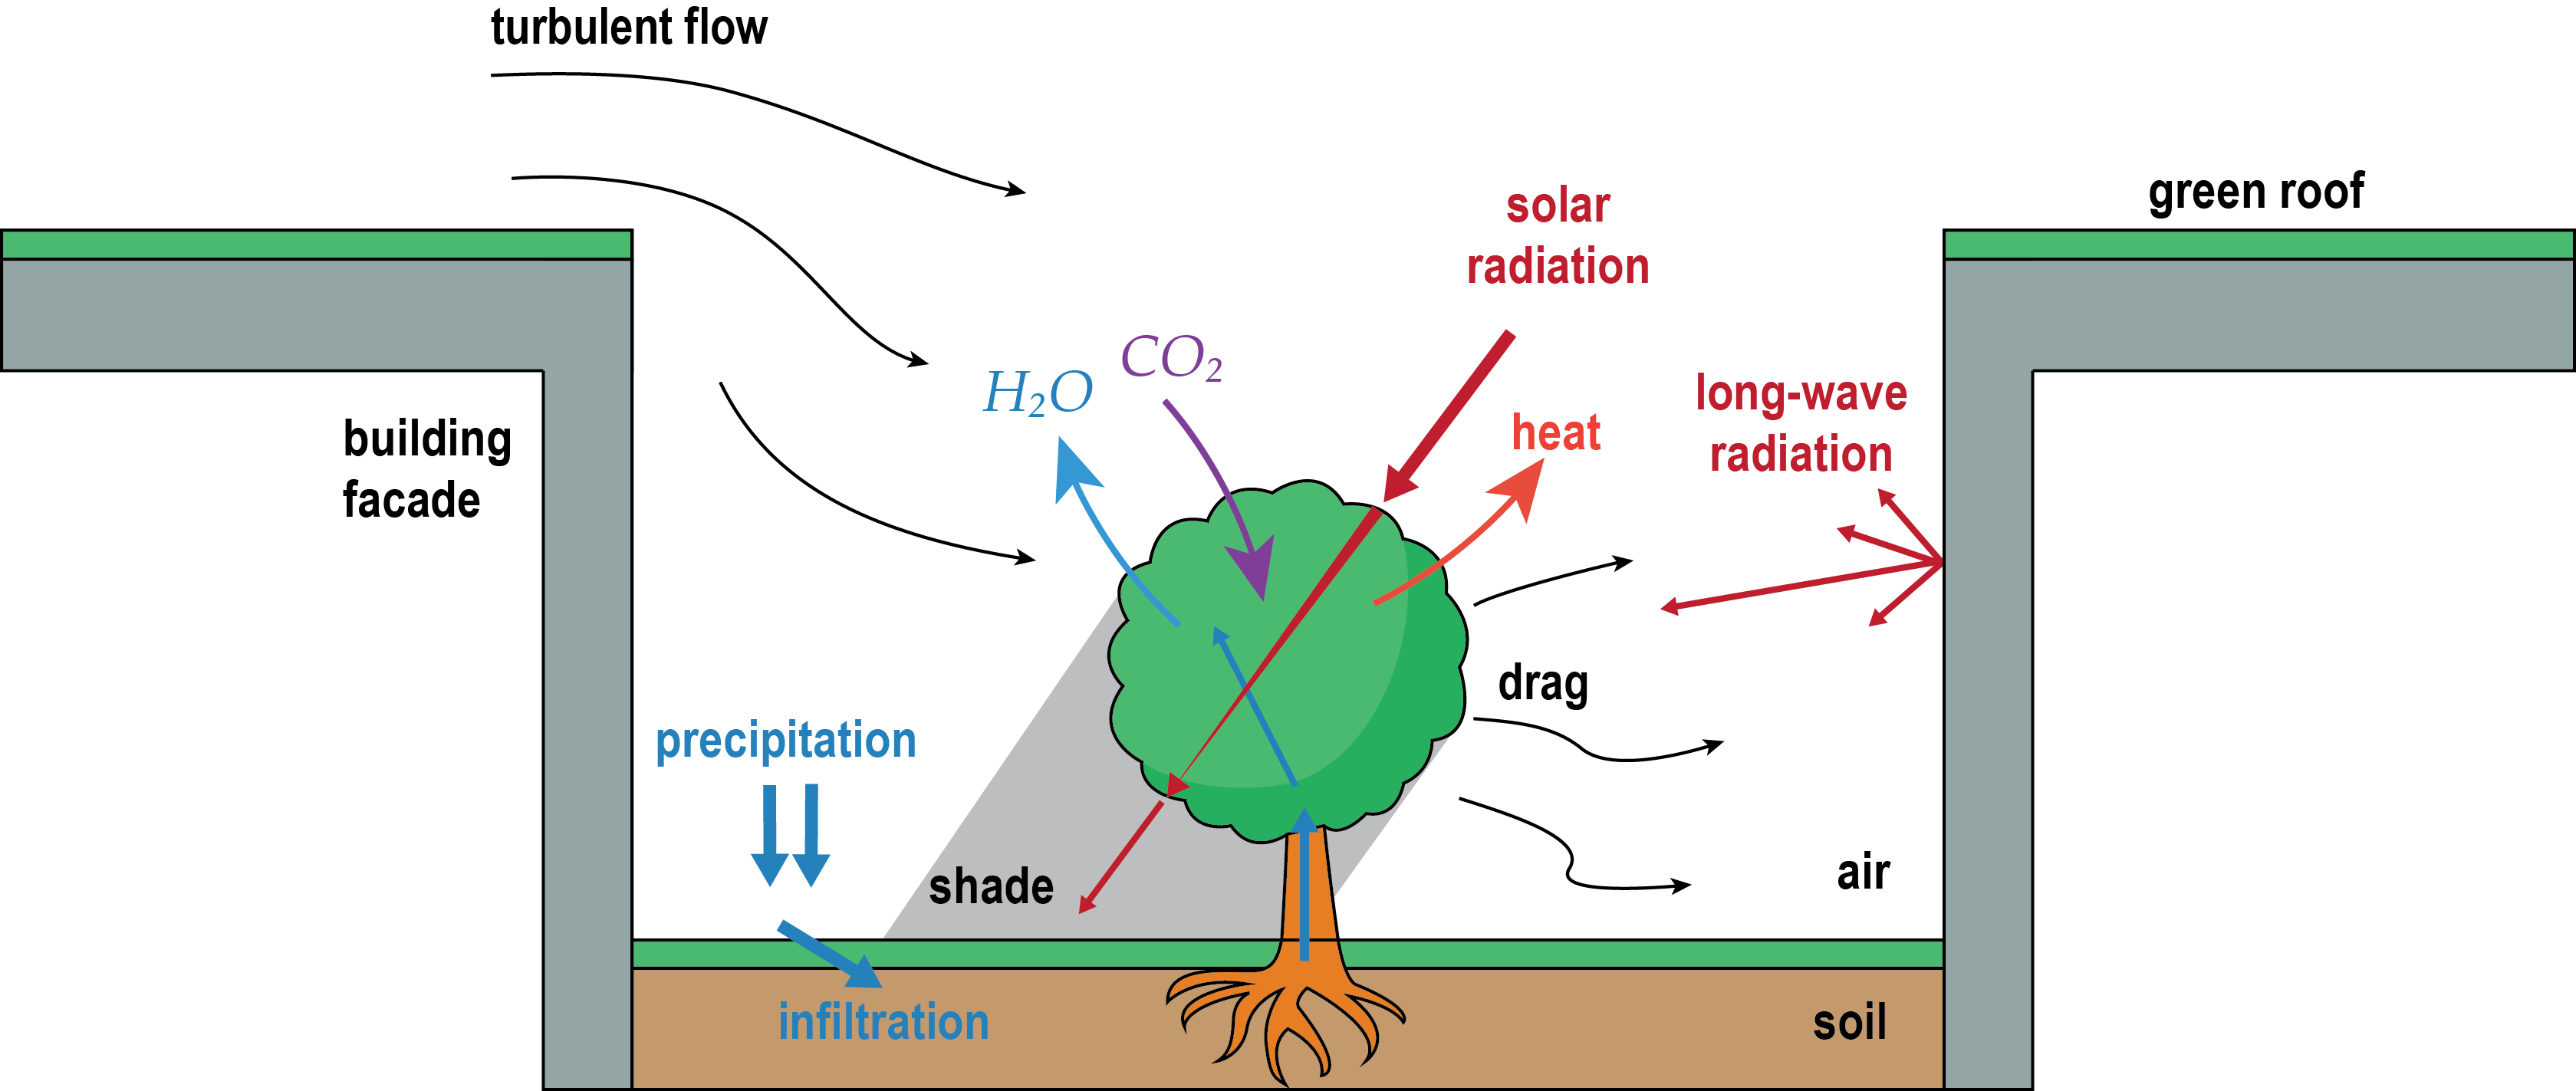
\includegraphics[width=\textwidth]{\figdir/streetcanyon_tree_part5.png}
	\caption{Impact of vegetation on urban microclimate.}
	\label{fig:vegetation_fluxes}
\end{figure}

Furthermore, due to the interception of solar radiation by the plant foliage, vegetation provides additional cooling from shading of nearby building elements. However, the moisture transpired by vegetation is also known to depend on the water availability. This indicates that the cooling potential of vegetation is dependent not only on the ambient atmospheric condition but also the soil moisture. Therefore, accurate predictions must take into account the hygrothermal characteristics of these domains (i.e., air and soil).

Therefore, there is a need for a multi-domain coupled numerical model that can take all these factors into account. Furthermore, the water cycle driven by the plant transpiration should be modeled to accurately assess the impact of vegetation on urban microclimate, especially the influence on thermal comfort. Furthermore, there is a great need for high-resolution data that can reveal the spatial and temporal variability in the plant responses. Wind tunnel experiment is known to be an effective tool in predicting and understanding urban flow phenomena using scaled models \citep{Allegrini2012,Paterna2015}. Typically, model trees are used to study the impact of vegetation in such urban geometry \citep{Gromke2008a}. Whether small model trees can accurately represent the aerodynamic characteristics of a mature tree still needs to be addressed. 

\section{Objective and Methodology}

Thus, the goal of the thesis is to improve the assessment of the impact of vegetation on the urban microclimate. As vegetation is increasingly being sought after as a natural UHI mitigation strategy, accurate predictions tools need to be available. More specifically, the objective of this thesis is as follows:
\begin{itemize}
	\item to assess the impact of vegetation on the microclimate.
	\item to quantify the natural cooling (i.e., transpirative cooling and shading) provided by vegetation in urban microclimate.
	\item to understand the influence of water stress on natural cooling.
	\item to quantify the impact of vegetation on pedestrian thermal comfort. 
\end{itemize}

In this thesis, experimental and numerical approaches are employed to assess the impact of vegetation on the microclimate. Experiments in an atmospheric boundary layer (ABL) wind tunnel are opted to understand the impact of vegetation on the airflow and the (near-wake) microclimate, where the small model and natural trees are employed as scaled models. Measurement techniques such as particle image velocimetry (PIV) and drag force measurement are employed to quantify the modification of airflow due to vegetation. Measurement techniques such as infrared thermography and hygrothermal sensor analysis are used to quantify the change in hygrothermal variables of the microclimate. A numerical assessment on the impact of vegetation on urban microclimate is achieved by integrating a vegetation model into a computation fluid dynamics (CFD) model in OpenFOAM. The developed numerical approach simultaneously resolves turbulence modification, radiation balance, heat and mass fluxes, and the sensitivity to soil moisture. The influence of the water availability on the transpiration rate is modeled using a soil-plant-atmosphere continuum (SPAC) model.  Thus, the model is to quantify the cooling potential of vegetation along with its impact on thermal comfort for a pedestrian.

\section{Outline of the thesis}

This thesis is divided into two parts: i) experimental studies (\cref{ch:paper2,ch:microclimatestudy}), and ii) numerical studies (\cref{ch:parametricstudy,ch:wtcfdcomparison,ch:numericalmethod,ch:impactofvegetation}) of the impact of vegetation on urban microclimate. The thesis is organized as follow:
\begin{itemize}
	\item \textit{Chapter 2}: The chapter addresses state of the art providing an overview on the urban climate, the impact of vegetation at microclimate scale, and typical experimental approaches and numerical approaches for assessing the impact of vegetation. The goal of the chapter is: i) to provide relevant researches that are present and are employed for quantifying the impact of vegetation on urban microclimate, ii) to provide a justification on the development of the numerical model that is presented in this thesis, and iii) to give the scope of the model. 

	\item \textit{Chapter 3}: This chapter is the first part of the experimental studies, where the impact of vegetation on the airflow is investigated. The influence of vegetation on the airflow is studied in an atmospheric boundary layer (ABL) wind tunnel using small model and natural trees. In the study, the turbulent airflow behind the trees is studied using particle image velocimetry (PIV) measurement technique and is linked to the drag force measurements using a load cell. The chapter has been published as: Manickathan, L., Defraeye, T., Allegrini, J., Derome, D., \& Carmeliet, J. (2018). ``Comparative study of flow field and drag coefficient of model and small natural trees in a wind tunnel''. \textit{Urban Forestry \& Urban Greening}, 230–239. \url{http://doi.org/10.1016/j.ufug.2018.09.011}.	

	\item \textit{Chapter 4}: This chapter is the second part of the experimental studies, where the impact of vegetation on the microclimate is investigated. The influence of vegetation on the microclimate is studied in the wind tunnel using a small \textit{Buxus sempervirens} plant. In the study, the diurnal dynamics of the plant microclimate of a \textit{Buxus sempervirens} is investigated using various high-resolution non-intrusive imaging techniques. The wake flow field is measured using stereoscopic particle image velocimetry (SPIV), the spatiotemporal leaf temperature history is obtained using infrared thermography, and the plant microstructure metrics such as plant porosity, leaf area density (LAD) is obtained through X-ray tomography.

	\item \textit{Chapter 5}: This chapter is the first part of the numerical studies, where the impact of vegetation on the transpirative cooling potential is investigated. The influence of vegetation on the transpirative cooling is studied using a computational fluid dynamics (CFD) modeling approach, where vegetation is modeled as a porous medium. In the chapter, a parametric study on the influence of environmental factors (i.e., wind speed, air temperature, relative humidity, and solar radiation intensity) and tree properties (i.e., leaf size, stomatal resistance, and leaf area density) on the transpirative cooling effect of trees is investigated. Furthermore, the Universal Thermal Climate Index (UTCI) around the trees is evaluated to determine the impact of transpirative cooling on pedestrian thermal comfort. The chapter has been published as: Manickathan, L., Defraeye, T., Allegrini, J., Derome, D., \& Carmeliet, J. (2018). ``Parametric study of the influence of environmental factors and tree properties on the transpirative cooling effect of trees''. \textit{Agricultural and Forest Meteorology}, 248, 259–274. \url{http://doi.org/10.1016/j.agrformet.2017.10.014}.

	\item \textit{Chapter 6}: This chapter is focuses on comparing the developed numerical in \cref{ch:parametricstudy} with the microclimate measurements of \cref{ch:microclimatestudy}. The goal of the chapter is to compare and determine the discrepancy of the numerical model in predicting the airflow and the transpiration cooling of vegetation. 

	\item \textit{Chapter 7}: This chapter the numerical model of assessing the impact of vegetation in urban microclimate is described. The \textit{air} domain solver, the \textit{solid} domain solver, and the \textit{radiation} model is described in detail. Furthermore, the chapter describes the coupling strategy employed to couple these three models with a detailed description of the coupling algorithm. The influence of water availability on transpiration rate is addressed by an advanced stomatal model based on the soil-plant-atmosphere continuum (SPAC) model approach. 

	\item \textit{Chapter 8}: This chapter is the second part of the numerical studies, where the impact of vegetation on the urban microclimate is investigated using the numerical model described in \cref{ch:numericalmethod}. The impact of vegetation on the urban microclimate consists of a modification to the turbulent urban airflow, the addition of transpirative cooling in the urban area, and the plant shading provided by the foliage. The influence of these phenomena is investigated together with the impact of pedestrian thermal comfort. 

	\item \textit{Chapter 9}: This chapter provides a conclusion and some of the main finding in the thesis. Furthermore, the chapter provides an overview of the contributions to the research field from the present thesis. Finally, an outlook and possible future research aspects are given.

	
\end{itemize}

